%%%%%%%%%%%%%%%%%%%%%%%%%%%%%%%%%%%%%%%%%%%%%%%%%%%%%%%%%%%%%%%%%%
% Artigo segundo as normais mais atualizadas da ABNT
% Adaptado do projeto ABNTeX2 (que nao esta totalmente sincronizada com as normas da ABNT)
% Autor: Berg Dantas (bergdantas@msn.com)
%%%%%%%%%%%%%%%%%%%%%%%%%%%%%%%%%%%%%%%%%%%%%%%%%%%%%%%%%%%%%%%%%%
\documentclass[article,12pt,oneside,a4paper,english,brazil,sumario=tradicional]{abntex2}		
% Pacotes usados
\usepackage{times}%Usa a fonte Latin Modern
\usepackage[T1]{fontenc}%Selecao de codigos de fonte.
\usepackage[utf8]{inputenc}%Codificacao do documento
\usepackage{indentfirst}%Indenta o primeiro parágrafo de cada seção.
\usepackage{nomencl}%Lista de simbolos
\usepackage{color}%Controle das cores
\usepackage{graphicx}%Inclusão de gráficos
\usepackage{microtype}%Para melhorias de justificação
\usepackage{lipsum}%Para geração de dummy text
\usepackage[abnt-emphasize=bf,abnt-and-type=e,alf]{abntex2cite}%Citações ABNT
\usepackage{mathptmx}
%\usepackage[bottom=2cm,top=3cm,left=3cm,right=2cm]{geometry}

% Configuracoes do documento
\graphicspath{{./imagens/}}%Images na pasta "Figuras"
\setsecheadstyle{\bfseries \normalsize \uppercase}
\setsubsecheadstyle{\normalsize \uppercase}
\setsubsubsecheadstyle{\bfseries \normalsize}
\setlrmarginsandblock{3cm}{2cm}{*}%Margens esquerda-direita
\setulmarginsandblock{3cm}{2cm}{*}%Margens cima-baixo
\checkandfixthelayout
\setlength{\parindent}{1.25cm}%paragrafo
\OnehalfSpacing%espacamento de 1,5
\setlength{\ABNTEXcitacaorecuo}{4cm}%recuo citacao direta +3

\begin{document}
\selectlanguage{brazil} % Seleciona o idioma do documento
\frenchspacing % Retira espaço extra obsoleto entre as frases.

\begin{center}
%TITULO
	\uppercase{\bfseries{Pulsares}}
	\vspace{12pt}
\end{center}

\begin{flushright}
%AUTOR - Pode-se contar com infinitos autores   :)
	Anthony Louis 17/0006239\footnote{UnB,17/0006239}
	\vspace{12pt}
\end{flushright}

\begin{footnotesize}
\SingleSpacing
\noindent
\small{\textbf{Resumo:}}
\noindent
\small
%TEXTO DO RESUMO (em português}
Esse artigo se trata de um trabalho para a disciplina de Fundamentos da Astronomia e Astrofísica, ministrada no período de verão de 2018. O temas a serem tratados são as principais características dos pulsares e o que faz desses elementos objetos fascinantes aos olhos dos Astrônomos.
\noindent
%PALAVRAS-CHAVE} 
\textbf{Palavras-chave}: Pulsares,Estrelas de Neutrôns,Quasares,Astronomia,Astrofísica.
\end{footnotesize}

\textual
\pagestyle{simple}
\aliaspagestyle{chapter}{simple}


\section{Estrelas}
\label{secIntroducao}
\normalsize
% TEXTO DA INTRODUCAO
Antes de explicar detalhadamente o conceito de um pulsar, deve-se explicar detalhadamente alguns conceitos importantes acerca das estrelas, principalmente sobre seu ciclo de vida.

Estrelas são bolas de plasma em quase equilíbrio hidrostático, formadas em grande parte por hidrogênio e hélio. Elas se formam a partir de nuvens frias de gases e poeira, através da interação gravitacional entre as partículas, as quais ao atingir certas condições físicas, conseguem se agrupar de modo a gerar a infinidade de estrelas observadas no meio celeste.

A principal característica que leva ao nascimento da estrela é o colapso de uma nuvem gasosa, devido à força gravitacional entre as partículas que a constitue. Isso ocasiona um processo de aquecimento, já que as partículas de poeira e gás ganham energia cinética nesse processo, que caso consiga elevar a temperatura da estrela até aproximadamente 8 milhões de Kelvin ($0,08 M_{sol}$ ), favorece o aparecimento de reações nucleares estáveis, as quais servirão de combustível para a estrela.

Nesse momento da evolução estelar, o estado de equilíbrio que permite a formação da estrela é garantido quando a pressão do gás que forma a estrela é aproximadamente igual à força gravitacional que une as moléculas, como mostra a imagem abaixo.

\begin{figure}[h]
	\centering
	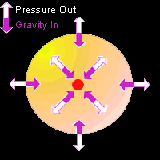
\includegraphics[]{estrelaformando.png}
\end{figure}

A partir desse ponto, grande parte das estrelas(mais de 90\%), as quais se encontram entre  $0,08M_{sol}$ e $8M_{sol}$, seguirão um ciclo de vida em que ocorrerá a transformação do hidrogênio em hélio a partir das reações de fusão e no final a estrela se tornará uma anã-branca. Deve-se ressaltar que o caminho até a estrela se tornar uma anã-branca depende da quantidade de massa presente na estrela.

Para estrelas com massas superiores a $0,45M_{sol}$, no fim de suas vidas,ocorre o processo de expansão até elas chegarem ao estágio de gigante vermelhas e, posteriormente, originando conchas gigantes de gases e plasma denominadas nebulosas planetárias. Por fim, elas finalizam seus ciclos de vida se transformando em anãs-brancas.

Nota-se que os objetos com massa menores que $0,08M_{sol}$ não conseguem alcançar o estágio que permite a ocorrência de reações nucleares estáveis. Portanto, acabam se tornando os outros objetos celestes visíveis no espaço, como anãs-marrom, planetas e asteroides. 

\begin{figure}[h]
	\centering
	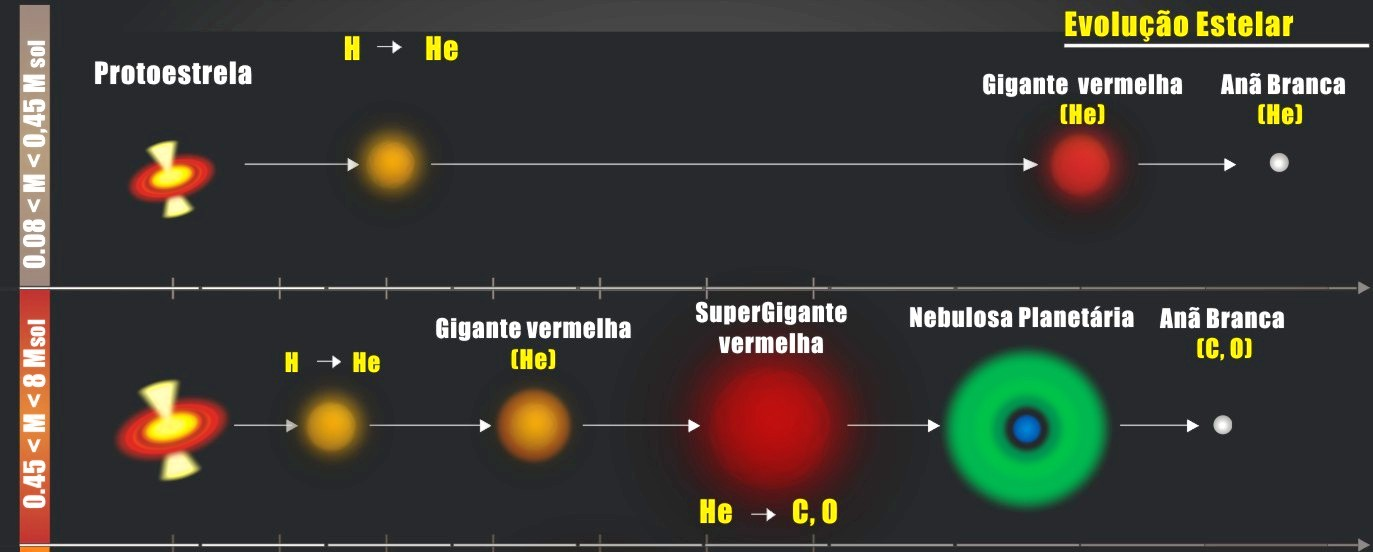
\includegraphics[width=1.0\linewidth]{evolucao_estrelas.jpg}
	\caption{Ciclo de vida de estrelas até $0,45M_{sol}$}
\end{figure}

\section{Estrelas Massivas}
A evolução das estrelas massivas, cuja massa é superior a $8M_{sol}$, decorre de modo diferente do explicitado no parágrafo anterior. Ao invés de apenas fazerem o estágio da fusão do hélio, seus núcleos atingem níveis de temperatura e pressão suficientes para realizarem a fusão de elementos mais pesados, como o Carbono, Oxigênio, Silício e Ferro.

Cada vez que a estrela começa a consumir um elemento mais pesado, ela realiza esse processo de forma mais rápida que o anterior.Assim, demora-se cerca de milhões de anos para efetuar a queima do hidrogênio em hélio, mas somente alguns minutos para efetuar a fusão do ferro no núcleo.Percebe-se nesse caso, a formação de diversas camadas na estrela, cada uma realizando a fusão de um elemento específico, desde o hidrogênio na parte externa ao ferro no núcleo da estrela.

Nesse ponto, deve-se ressaltar que devido ao fato da fusão do ferro ser endotérmica, não há a fusão de elementos mais pesados que ele no ciclo de vida das estrelas.

Com o aumento da fusão de ferro no núcleo estelar, o combustível de manutenção dela começa a se extinguir, os processos intranucleares absorvem mais energia, o que torna a estrela cada vez mais fria, à medida que ela se expande.Esses eventos causam a redução da pressão do objeto e acelera o colapso gravitacional do núcleo, com isso a estrela entra em um processo onde as camadas externas começam a contrair em direção ao núcleo.

No núcleo, ocorre o aumento intenso do número de nêutrons a partir da fotodesintegração do ferro em elementos menores e a partir da degeneração de elétrons e prótons, que geram neutrôns em uma reação exotérmica(p + e = n + v). Com isso, a contração sofrida nas camadas externas da estrela ricocheteia no núcleo e retorna em uma expansão violenta, ejetando matéria(neutrinos,elétrons..) e energia no espaço, com um brilho extremamente alto e formação de elementos bem mais pesados que o ferro.

Esse processo descrito é denominado supernova e marca o fim da vida dos objetos estelares, quando o combustível que os sustentava se esgota. Para estrelas massivas, esse tipo de supernova descrito é o "Type II".

\begin{figure}[h]
	\centering
	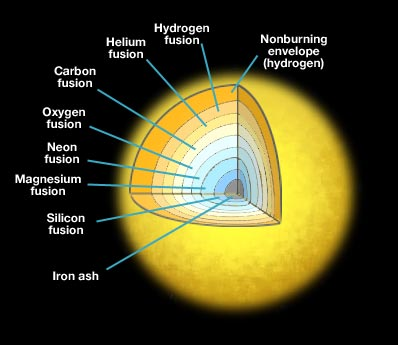
\includegraphics[height=7cm]{supernova.jpg}
	\caption{Camadas em uma estrela massiva}
\end{figure}
 
\section{Estrelas de Neutrôns}

Depois do processo de supernova descrito no parágrafo anterior, para estrelas com massa até $25M_{sol}$, sobra apenas uma bola compacta de 20 km de diâmetro com massa de aproximadamente $1,4M_{sol}$, composta de neutrôns extramamente comprimidos.

Devido ao seu pequeno tamanho e grande massa, esses objetos possuem um campo gravitacional na superfície com o valor $2\cdot 10^{11}$ vezes o  da Terra. Além de um campo eletromagnético milhões de vezes mais forte que o encontrado no planeta Terra.

Esse conjunto de fatores faz com que a estrela de neutrôns seja capaz de realizar fenômenos interessantes, como a Lente Gravitacional: onde o campo gravitacional dela distorce o espaço-tempo próximo, causando desvios nas trajetórias da luz que passam próximos dali. Outros dois fenômenos importantes são o fato de estrelas de neutrôns adquirirem,devido à sua força gravitacional, um grande momento angular, girando várias vezes por segundo e  o fato delas expulsarem jatos de matéria em alta velocidade pelos seus polos magnéticos.

Deve-se ressaltar que,assim como a Terra, os eixos de rotação e os polos magnéticos das estrelas de neutrôns estão desalinhados. 

\begin{figure}[h]
	\centering
	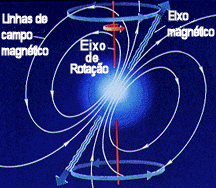
\includegraphics[height=5cm]{modelopulsar.png}
	\caption{Estrela de neutrôns}
\end{figure}

\section{Pulsares}
Quando moléculas de corpos supermassivos fluem em direção às estrelas de neutrôns e entram em contato com o seu campo magnético, essa interação provoca os jatos que são expelidos pelos polos da estrela.

Esses jatos podem ser visualizados nas bandas de rádio, óptico, raios-x ou raios-gama. Quando eles estão na direção da Terra, sua aparência se torna como uma lâmpada de um farol aceso para os observadores terrestres.

Contudo, devido a alta rotação dessas estrelas e o desalinhamento dos polos magnéticos com o eixo de rotação, os jatos entram e saem da direção da Terra, o que gera pequenos pulsos de energia que são capturados pelos astrônomos.

Por isso, essas estrelas de neutrôns em rotação e campo magnético extremamente altos são denominados pulsares, sendo que os pulsos detectados são extremamente regulares no tempo. Logo, todos os pulsares são de fatos estrelas de neutrôns, embora nem toda estrela de neutrôn seja um pulsar. 

A primeira detecção de um pulsar se deu pelos astrônomos Jocelyn Bell e Antony Hewish em Cambridge no ano de 1967. Esses sinais foram obtidos na banda de rádio com uma frequência de 1,33 segundos e duração de 0,04 segundos, vindos da constelação de Vupércula. Contudo, eles dois acreditaram  que a força e a regularidade desse sinal seria uma tentativa de comunicação extraterrestre, apelidando assim o objeto de \textit{Little Green Man}(Pequeno Homem Verde) em alusão a esse pensamento.

Apenas posteriormente, o polêmico astrônomo Thomas Gold desenvolveu a explicação correta para o fenômeno dos pulsares. Ele argumentou que se tratavam de estrelas de neutrôns que emitiam energia ao passo que se encontravam em um estado imenso de rotação. Essa teoria incialmente foi considerada demasiada absurda e apenas com a descoberta da Nebulosa de Carangueijo que ela passou a ser aceita pela comunidade científica.

\begin{figure}[h]
	\centering
	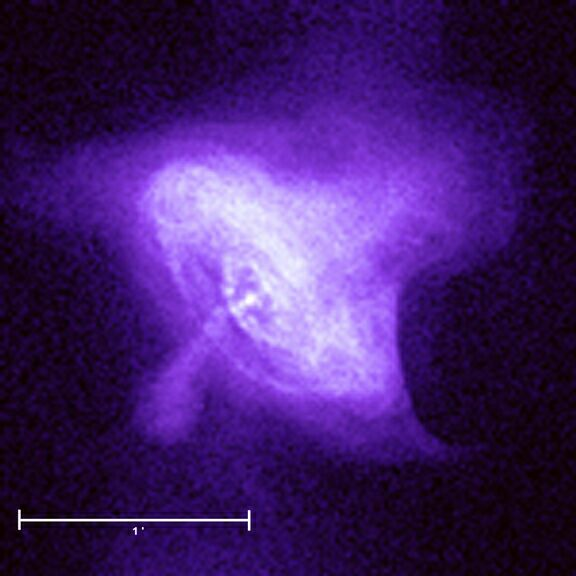
\includegraphics[width=0.6\linewidth,height=5cm]{crab2pul.jpg}
\end{figure}

Em 1974, Hewish ganhou o prêmio Nobel devido às suas descobertas no campo dos pulsares e radioastronomia, junto com Martin Ryle. Contudo, houve uma certa exclusão das contribuições de Jocelyn Bell, que ajudou na construção dos telescópios, reportou erros e foi responsável pela descoberta do pulsar. Esse fato até hoje é considerado uma das maiores controvérsias do Prêmio Nobel.

\section{Pulsares Importantes}
Segue abaixo a lista dos pulsares mais famosos na literatura astronômica:
\begin{description}
	\item[PSR B1919 + 21.:] primeiro pulsar descoberto na história, por Jocelyn Bell em 1967, com frequência de aproximadamente 1,33s e apelidado de LGM-1;
	\item[Crab Pulsar:] resultante de uma explosão de supernova. Um dos objetos mais bem conhecidos e estudados do cosmos, encontrando-se dentro da nebulosa de mesmo nome e brilhando em quase todo espectro eletromagnético;
	\item[PSR J0540-6919:] encontra-se a 163000 anos-luz de distância, sendo o primeiro além de nossa galáxia a ser encontrado emitindo em raios-gama e o mais brilhante nessa banda;
	\item[IGR J18245-2452:] pulsar de "dupla indentidade", descoberto em 2013, que se alterna na emissão de raios-x e ondas de rádio;
	\item[PSR J1023 + 0038:] pulsar encontrado em 2013 que sofre uma transformação devido a sua estrela companheira. Quando foi visualizado estava emitindo em rádio quando de repente desapareceu e pulsou cinco vezes em raios gama, como se alguém tivesse ativado um interruptor para aumentar a energia.
\end{description}

\section*{Referências}
http://www.skyandtelescope.com/astronomy-resources/what-is-a-star/

http://www.ccvalg.pt/astronomia/nebulosas/nebulosas- planetarias.htm

https://www.nasa.gov / audience/ forstudents/9-12/features stellar-evol-feat-912.html

http://astro.if.ufrgs.br/estrelas/evolucao-estrelas.jpg

https://books.google.com.br/

http://www.iaea.org/inis/collection/NCLCollectionStore/-Public /  43/058/43058375.pdf

https://www.e-education.psu.edu/astro801/content/l6-p5.html

https://edisciplinas.usp.br/pluginfile.php/cap15a-evol-massivas.pdf

http://www.solstation.com/x-objects/crab-neb.htm

http:innovacionespacial.blogspot.com.br/cinco-famosos-pulsares-de-los-ultimos.html

http://astro.if.ufrgs.br/estrelas/node14.htma

http://www.astropt.org/2017/07/09/o-que-sao-os-pulsares/

http://www.if.ufrgs.br/mpef/mef008/trabalhos-03/Pulsares.htm

https://imagine.gsfc.nasa.gov/science/objects/pulsars1.html.old

https://www.space.com/22180-neutron-stars.html
\end{document}